\documentclass{beamer}

\usepackage{graphicx}
\usepackage{hyperref}
\usepackage[latin1]{inputenc}
\usepackage[T1]{fontenc}
\usepackage[english]{babel}
\usepackage{listings}
\usepackage{xcolor,mathrsfs,url}
\usepackage{amssymb}
\usepackage{amsmath}
\usepackage{ifthen}

% The command to define a subsection is '\subsec{}' and NOT '\subsection'.
% This code generates the bar. Don't edit.
\newcommand{\midbarnew}{}
\newcommand{\subsec}[1]
{
  \ifthenelse{\equal{#1}{}}
  {\renewcommand{\midbarnew}{} \subsection{}}
  {\renewcommand{\midbarnew}{ $\mid$ } \subsection{#1}}
}

% change the pictures here, if necessary. logobig and logosmall are the internal names
% for the pictures: do not modify them, just change "hulogo" and "logo". Pictures must be 
% supplied as JPEG, PNG or PDF
%########################################

% \pgfdeclareimage[height=2cm]{logobig}{logo} % use hucase instead for the Humboldt-Case Logo
% \pgfdeclareimage[height=1cm]{logosmall}{logo}

% use this number to modify the scaling of the headline on titlepage

\title{Trade Policy: Part One}
\author{Instructor: David Jinkins\thanks{I wish to acknowledge Battista Severgnini for providing last year's slides to me. His generosity saved me much time, and these slides are partially based on his. Any errors are of course my own.}}
\date{Date: Sept. 23, 2014}

%Start of the document
\begin{document}

\frame{\titlepage}

\begin{frame}
    \begin{itemize}
    \itemsep1pt\parskip0pt\parsep0pt
    \item
      Last time: Increasing Returns to Scale
      \begin{itemize}
            \item Krugman: External Economies 
            \begin{itemize}
                \item Larger industries have lower cost
                \item Drives industries to concentrate
                \item A reason for trade
            \end{itemize}
            \item Implications of external economies 
            \begin{itemize}
                \item Historical Accident
                \item Money on the table
                \item Infant industries
            \end{itemize}
            \item Melitz and Krugman: Internal Economies
            \begin{itemize}
                \item Larger firms have lower cost 
                \item Each firm a different product or variety
                \item Consumers like a mix
                \item Reason for trade: more (and cheaper) varieties
            \end{itemize}
        \end{itemize}
    \end{itemize}
\end{frame}

\frame{% how to print
\frametitle{Plan for Today}
Chapter 8:
\begin{itemize}
\item Review: Monopoly
\item Review: Monopolistic competition
\item New: Trade costs
\item New: Dumping
\item New: Multinationals
\end{itemize}
Chapter 9 : 
\begin{itemize}
\item Tariffs
\item Consumer \& Producer Surplus
\item Export Subsidies
\end{itemize}
Chapter 10 :
}

\begin{frame}{Review}
    \begin{itemize}
        \item Begin review
    \end{itemize}
\end{frame}

\frame[plain]{
\includegraphics[page=26,width=\textwidth]{scale_and_trade.pdf}}
\frame[plain]{
\includegraphics[page=27,width=\textwidth]{scale_and_trade.pdf}}
\frame[plain]{
\includegraphics[page=32,width=\textwidth]{scale_and_trade.pdf}}
\frame[plain]{
\includegraphics[page=33,width=\textwidth]{scale_and_trade.pdf}}
\frame[plain]{
\includegraphics[page=34,width=\textwidth]{scale_and_trade.pdf}}
\frame[plain]{
\includegraphics[page=35,width=\textwidth]{scale_and_trade.pdf}}
\frame[plain]{
\includegraphics[page=37,width=\textwidth]{scale_and_trade.pdf}}
\frame[plain]{
\includegraphics[page=38,width=\textwidth]{scale_and_trade.pdf}}
\frame[plain]{
\includegraphics[page=39,width=\textwidth]{scale_and_trade.pdf}}
\frame[plain]{
\includegraphics[page=40,width=\textwidth]{scale_and_trade.pdf}}
\frame[plain]{
\includegraphics[page=41,width=\textwidth]{scale_and_trade.pdf}}
\frame[plain]{
\includegraphics[page=43,width=\textwidth]{scale_and_trade.pdf}}
\frame[plain]{
\includegraphics[page=44,width=\textwidth]{scale_and_trade.pdf}}
\frame[plain]{
\includegraphics[page=46,width=\textwidth]{scale_and_trade.pdf}}
\frame[plain]{
\includegraphics[page=47,width=\textwidth]{scale_and_trade.pdf}}
\frame[plain]{
\includegraphics[page=48,width=\textwidth]{scale_and_trade.pdf}}
\frame[plain]{
\includegraphics[page=51,width=\textwidth]{scale_and_trade.pdf}}
\frame[plain]{
\includegraphics[page=52,width=\textwidth]{scale_and_trade.pdf}}
\frame[plain]{
\includegraphics[page=53,width=\textwidth]{scale_and_trade.pdf}}
\frame[plain]{
\includegraphics[page=54,width=\textwidth]{scale_and_trade.pdf}}
\frame[plain]{
\includegraphics[page=57,width=\textwidth]{scale_and_trade.pdf}}
\frame[plain]{
\includegraphics[page=58,width=\textwidth]{scale_and_trade.pdf}}
\frame[plain]{
\includegraphics[page=59,width=\textwidth]{scale_and_trade.pdf}}
\frame[plain]{
\includegraphics[page=60,width=\textwidth]{scale_and_trade.pdf}}
\frame[plain]{
\includegraphics[page=63,width=\textwidth]{scale_and_trade.pdf}}
\frame[plain]{
\includegraphics[page=67,width=\textwidth]{scale_and_trade.pdf}}
\frame[plain]{
\includegraphics[page=68,width=\textwidth]{scale_and_trade.pdf}}
\frame[plain]{
\includegraphics[page=70,width=\textwidth]{scale_and_trade.pdf}}
\frame[plain]{
\includegraphics[page=72,width=\textwidth]{scale_and_trade.pdf}}

\begin{frame}
    \begin{itemize}
        \item End review!
    \end{itemize}
\end{frame}

\begin{frame}{Trade Costs and Extensive Margin} 
    \begin{itemize}
        \item Suppose there is some cost to trade 
        \item Equivalent to increasing marginal cost of production
        \item Recall firms with high marginal cost don't enter domestic market 
        \item Even fewer firms will enter the export market
        \item \emph{Extensive margin}: Number of firms exporting
        \item \emph{Intensive margin}: How much each firms export
        \item Trade costs reduce both
    \end{itemize}
\end{frame}

\begin{frame}{Extensive Margin is important} 
    \begin{itemize}
        \item Small share of firms export -- 18\% of American firms overall 
    \end{itemize}
    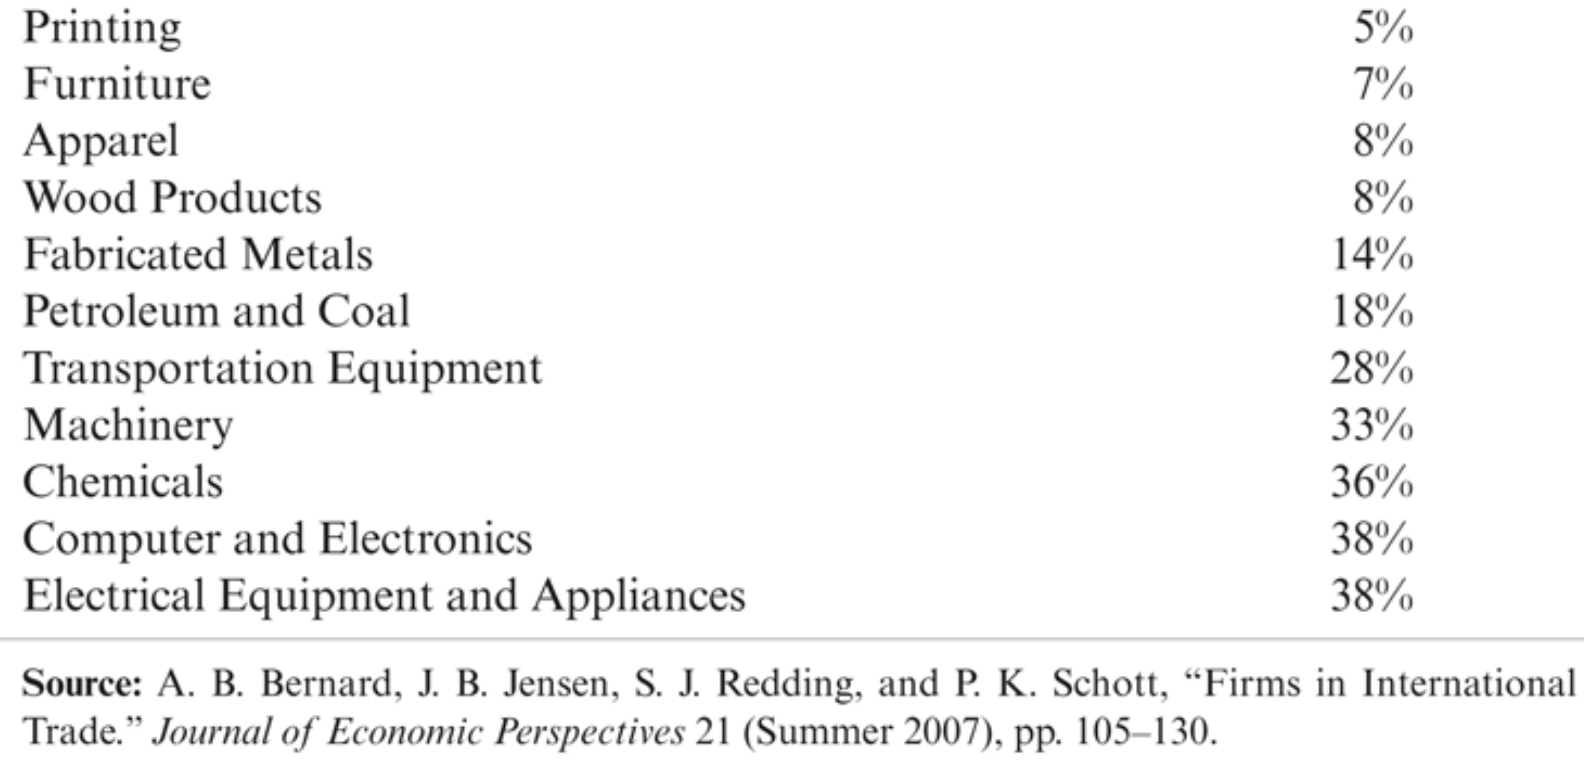
\includegraphics[scale=0.20]{bjrs_firms.png}
\end{frame}

\begin{frame}{Extensive Margin in a Picture} 
    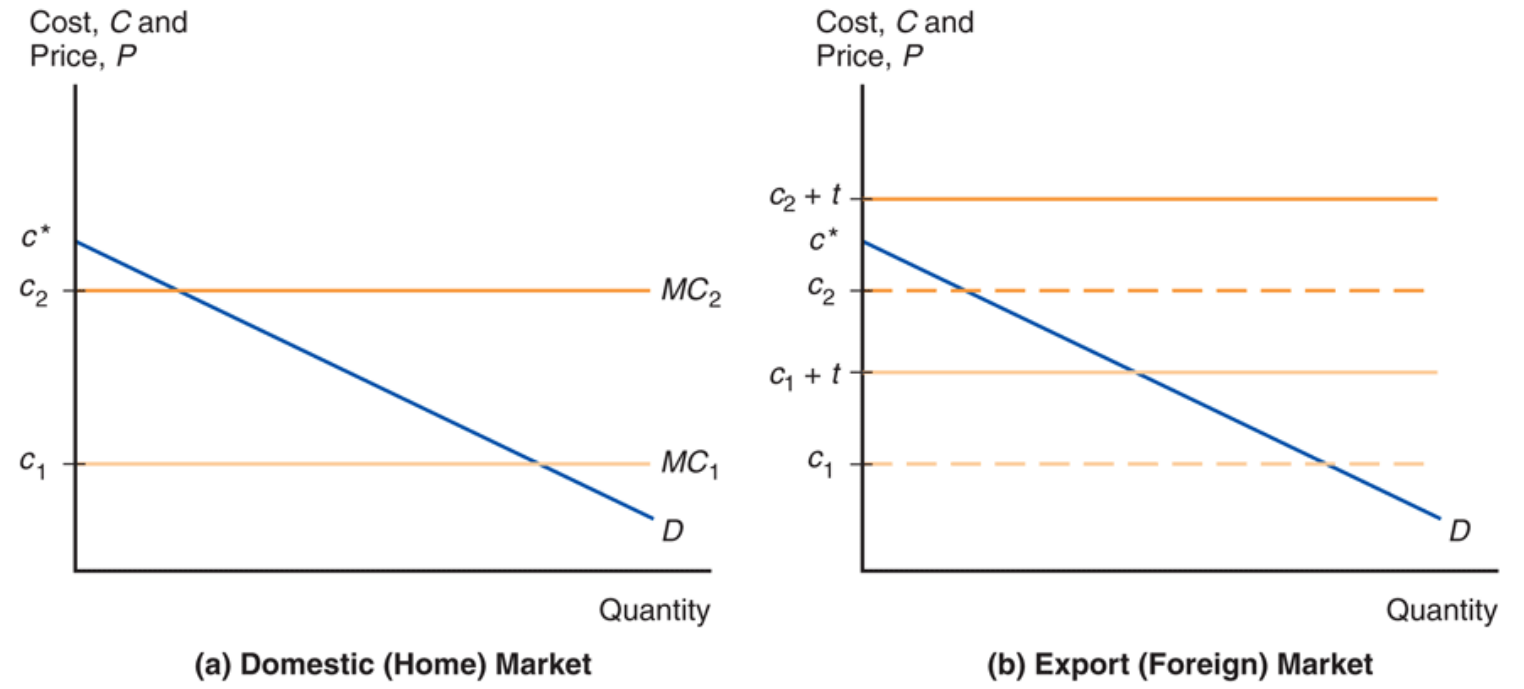
\includegraphics[scale=0.20]{trade_costs_firms.png}
\end{frame}

\begin{frame}{Predictions of Heterogenous Firms with Trade Cost}
    \begin{itemize}
        \item Subset of firms export
        \item Those that do are relatively productive
        \item Largely backed up by data:
        \begin{itemize}
            \item Exporters on average twice as large as importers (size vs. prod?)
            \item Produce on average 11\% more per worker
        \end{itemize}
    \end{itemize}
\end{frame}

\begin{frame}{Dumping}
    \begin{itemize}
        \item \emph{Dumping} is when a firm sells a product too cheaply abroad
        \begin{enumerate}
            \item Sometimes if foreign price below domestic price 
            \item Sometimes if foreign price below domestic price plus tariff
            \item Sometimes if foreign price is below cost of production
        \end{enumerate}
        \item Considered an unfair trade practice, WTO allows 'antidumping duty' or tariff
        \item Monopolistic competitive firms naturally do No. 2 (but not No. 1 or No. 3)
        \item Why?
        \item Textbook: This is just natural firm behavior 
        \item Me: Don't feel too bad -- these firms are still monopolists!
    \end{itemize}
\end{frame}

\begin{frame}{Pause}

    \begin{itemize}
        \item Trade costs: exporters on average more productive
        \item Dumping: Depending on definition, natural behavior
        \item Now: Foreign Direct Investment
        \item Note: Not directly related to increasing returns
        \item Included because firm behavior in trade
    \end{itemize}

\end{frame}

\begin{frame}{Foreign Direct Investment}

    \begin{itemize}
        \item Comes in two flavors
        \begin{enumerate}
            \item \emph{Vertical}: Do manufacturing where it is cheap
            \item \emph{Horizontal}: Produce close to final market
        \end{enumerate}
        \item Vertical example: iPhones made in China, designed in California
        \item Horizontal example: Japanese cars produced in the United States
    \end{itemize}

\end{frame}

\begin{frame}{Motives for FDI}
    \begin{itemize}
        \item Vertical FDI
        \begin{itemize}
            \item ex: Take advantage of lower labor costs abroad
            \item Capital can move: Factor price equalization all over again!
        \end{itemize}
        \item Horizontal FDI
        \begin{itemize}
            \item Proximity-Cost tradeoff
            \item Language developed by my professor, Steven Yeaple (along with Melitz)
            \item Low transport cost, export more
            \item High transport cost, build factor abroad
            \item Prediction consistent with data
        \end{itemize}
    \end{itemize}
\end{frame}

\begin{frame}{Outsourcing and Offshoring}
    \begin{itemize}
        \item In both flavors of FDI, keep transactions in the firm?
        \item Vertical
        \begin{itemize}
            \item Should you buy intermediates from foreign frim?
            \item Or build a factor abroad?
        \end{itemize}
        \item Horizontal
        \begin{itemize}
            \item Should you license technology to local producer?
            \item Or open a foreign factory yourself?
        \end{itemize}
        \item These are deep and difficult questions
        \item Depend on the theory of the firm
        \begin{itemize}
            \item Economics about the power of the market
            \item Each firm is a tiny communist country 
        \end{itemize}
    \end{itemize}
\end{frame}

\begin{frame}{Offshoring increasingly important}

    \begin{itemize}
        \item Intermediates are 40\% of manufactures trade (which are around 55\% of world trade)
        \item Intra-firm trade is 30\% of world trade
        \item Frontier of research, no definitive motive for internalization
    \end{itemize}

\end{frame}

\begin{frame}{Chapter 8: Summary}

    \begin{itemize}
        \item Monopolistic Competition
        \item Fixed cost give increasing return to scale
        \item Model for analyzing firms and trade (why?)
        \item Trade grows productive firms, shrinks unproductive firms
        \item Effect like productivity growth
        \item Frontier of research: FDI and internalization decisions
    \end{itemize}

\end{frame}
% \frame{% how to print

% \frametitle{}
% \begin{center}
% \textcolor{blue}{\Huge{\textbf{Chapter 9: The Instruments of Trade Policy}}}
% \end{center}
% }
% 
% \frame{
% \frametitle{Chapter 9-11}
% \begin{itemize}
% \item First 8 chapters: \textit{Why do countries trade?}
% \item Chapters 9-12: \textit{What should a nation's trade policy
% be?}
% \end{itemize}
% }
% 
% \frame{
% \frametitle{Purpose of Trade Policy}
% Governments use instruments of trade policy to protect domestic industries that would result from
% import competition.
% }
% 
% \frame{
% \frametitle{Purpose of Trade Policy}
% President George W. Bush
% \begin{itemize}
% \item \textbf{March 5th, 2002, announcing new "safeguards" tariffs on imported steel:} \textit{I take this action to give our domestic steel industry an opportunity to adjust to surges in foreign imports, recognizing the harm from 50 years of foreign government intervention in the global steel market.}
% \item \textbf{December 4th, 2003, announcing the removal of the "safeguards" tariffs on imported steel:} \textit{I took action to give the industry a chance to adjust to the surge in foreign imports and to give relief to the workers and communities that depend on steel for their jobs and livelihoods. The safeguard measures have now achieved their purpose, and a result of changed economic circumstances, it is time to lift them.}
% \end{itemize}
% }
% 
% \frame{
% \frametitle{Tariffs (1)}
% Two types of tariffs:
% \begin{enumerate}
% \item \textbf{specific tariff:} fixed charge for each \textit{unit} of imported goods (e.g., 1 DKK per kg of cheese)
% \begin{center}
% $P=P^{*}+t$
% \end{center}
% \item \textbf{\textit{ad valorem} tariff:} fraction of the \textit{value} of imported goods (e.g., 25\% tariff on the value of imported cars) 
% \begin{center}
% $P=P^{*}\left(1+\tau\right)$
% \end{center}
% \end{enumerate}
% }
% 
% \frame{
% \frametitle{Tariffs (2): A Model}
% How does a tariff affect a single market?
% \begin{itemize}
% \item \textit{partial equilibrium framework} (reasonable for understanding trade policies towards one sector)
% \item assumption: $P^{WHEAT}>P^{*WHEAT}$
% \item with trade: $P^{WHEAT}>P>P^{*WHEAT}\Rightarrow$ H imports the good, while F
% exports it.
% \end{itemize}
% }
% 
% \frame{
% \frametitle{Import Demand Curve}
% The import demand curve for H (MD) is the difference between the quantity that domestic consumers demand minus the quantity that domestic producers supply, at each price.
% }
% 
% 
% \frame{
% \frametitle{Fig. 9-1: Deriving Home's Import Demand Curve}
% \begin{figure}
% 	\centering
% 		\includegraphics[width=0.80\textwidth]{81.pdf}
% 	\label{fig:11}
% \end{figure}
% }
% 
% \frame{
% \frametitle{Export Supply Curve}
% The export supply curve for F (XS) is the difference between the quantity that foreign producers supply minus the quantity that foreign consumers demand, at each price.
% }
% 
% \frame{
% \frametitle{Fig. 9-2: Deriving Foreign�s Export Supply Curve}
% \begin{figure}
% 	\centering
% 		\includegraphics[width=0.80\textwidth]{82.pdf}
% 	\label{fig:11}
% \end{figure}
% }
% 
% \frame{
% \frametitle{World Market Equilibrium}
% Combine XS and MD curves: equilibrium price and quantity at
% the world market.
% In equilibrium
% \begin{itemize}
% \item import demand = export supply
% \item domestic demand -� domestic supply =foreign supply -� foreign demand ($D-S=S^{*}-D^{*}$)
% \item world demand = world supply ($D+D^{*}=S^{*}-S$)
% \end{itemize}
% }
% 
% \frame{
% \frametitle{Fig. 9-3: World Equilibrium}
% \begin{figure}
% 	\centering
% 		\includegraphics[width=0.80\textwidth]{83.pdf}
% 	\label{fig:11}
% \end{figure}
% }
% 
% \frame{
% \frametitle{The Effects of a Tariff}
% \begin{itemize}
% \item A tariff can be viewed as an added cost of transportation, making sellers unwilling to ship goods unless the price difference between the domestic and foreign markets exceeds the tariff.
% \item Introduce a tariff $t$
% \begin{center}
% $P_{T} = P^{*}_{T} + t \Rightarrow P^{*}_{T} =P_{T} -� t$
% \end{center}
% \item Only part of the tariff is past on to H consumers:
% \begin{enumerate}
% \item $t\Uparrow\Rightarrow P_{T}\Uparrow: S\Uparrow, D\Downarrow\Rightarrow MD \Downarrow$
% \item $t\Uparrow\Rightarrow P^{*}_{T}\Downarrow: S\Downarrow, D\Uparrow\Rightarrow XS \Downarrow$
% \end{enumerate}
% \end{itemize}
% }
% 
% \frame{
% \frametitle{Fig. 9-4: Effects of a Tariff}
% \begin{figure}
% 	\centering
% 		\includegraphics[width=0.80\textwidth]{84.pdf}
% 	\label{fig:11}
% \end{figure}
% }
% 
% 
% \frame{
% \frametitle{The Effects of a Tariff in a Small Country}
% \begin{itemize}
% \item When a country is \textit{small}, tariff $t$ has no effect on the foreign (world) price of a good, because its demand of the good is an insignificant part of world demand.
% \item the full tariff is passed
% on to consumers.
% \end{itemize}
% }
% 
% \frame{
% \frametitle{Fig. 9-5: A Tariff in a Small Country}
% \begin{figure}
% 	\centering
% 		\includegraphics[width=0.80\textwidth]{85.pdf}
% 	\label{fig:11}
% \end{figure}
% }
% 
% 
% \frame{
% \frametitle{Costs and Benefits of Tariffs}
% \begin{itemize}
% \item A tariff raises the price of a good in the importing country, so we expect it to hurt consumers and benefit producers there.
% \item In addition, the government gains tariff revenue from a tariff.
% \end{itemize}
% }
% 
% \Section{Chapter 9. Consumer \& Producer Surplus}
% 
% \frame{
% \frametitle{Consumer Surplus (1)}
% Consumer surplus measures the amount that consumers gain from purchases by the difference in the price that each pays from the maximum price each would be willing to pay.
% }
% 
% \frame{
% \frametitle{Consumer Surplus (2)}
% \begin{figure}
% 	\centering
% 		\includegraphics[width=0.80\textwidth]{cs1.pdf}
% 	\label{fig:11}
% \end{figure}
% }
% 
% 
% \frame{
% \frametitle{Producer Surplus}
% \begin{figure}
% 	\centering
% 		\includegraphics[width=0.80\textwidth]{ps1.pdf}
% 	\label{fig:11}
% \end{figure}
% }
% 
% 
% \frame{
% \frametitle{How is Welfare affected by $t$?}
% \begin{itemize}
% \item Gains to domestic producers
% \begin{center}
% $\Delta PS=a$
% \end{center}
% \item Loss to domestic consumers:
% \begin{center}
% $\Delta CS=\left(a+b+c+d\right)$
% \end{center}
% \item Government revenue:
% \begin{center}
% $\Delta R=\left(c+e\right)$
% \end{center}
% \item Total net loss (can be positive or negative):
% \begin{center}
% $\Delta PS-\Delta CS-\Delta R\right$=
% \end{center}
% \begin{center}
% $\left(a+b+c+d\right)-a-\left(c+e\right)$=
% \end{center}
% \begin{center}
% $=b+d-e$
% \end{center}
% \end{itemize}
% }
% 
% 
% \frame{
% \frametitle{Fig. 9-9: Costs and Benefits of a Tariff for the Importing Country}
% \begin{figure}
% 	\centering
% 		\includegraphics[width=0.80\textwidth]{85bis.pdf}
% 	\label{fig:11}
% \end{figure}
% }
% 
% 
% 
% \frame{
% \frametitle{Measures $b$, $d$ and $e$}
% \begin{itemize}
% \item $b$ production distortion, $d$ consumption
% distortion $\Rightarrow$ efficiency loss
% \item $t$ distorts incentives of both consumers and
% producers by inducing them to act as if
% imports were more expensive that it actually
% are.
% \item produces extra units of the good that could
% be produced cheaper abroad
% \item consumes less units of the good that could
% be bought cheaper abroad
% \item $e$ terms of trade gain
% \end{itemize}
% }
% \frame{
% \frametitle{Fig. 9-10: Net Welfare Effects of a Tariff}
% \begin{figure}
% 	\centering
% 		\includegraphics[width=0.80\textwidth]{86.pdf}
% 	\label{fig:11}
% \end{figure}
% }
% 
% 
% \frame{
% \frametitle{Costs and Benefits of Tariffs (1)}
% \begin{itemize}
% \item The triangles $b$ and $d$ represent the efficiency loss
% \item The rectangle $e$ represents the terms of trade gain. 
% \end{itemize}
% }
% 
% \end{document}
% \Section{Chapter 9. Export Subsidies}
% \frame{
% \frametitle{Export Subsidies (1)}
% Two types of export subsides:
% \begin{enumerate}
% \item \textbf{specific subsudy:} a payment per unit exported.
% \item \textbf{\textit{ad valorem} subsidy:} payment as a proportion of the value exported. 
% \end{enumerate}
% }
% 
% \frame{
% \frametitle{Export Subsidies (2)}
% \begin{itemize}
% \item An export subsidy raises the price of a good in the exporting country, while lowering it in foreign countries.
% \item In contrast to a tariff, an export subsidy worsens the terms of trade by lowering the price of domestic products in world markets.
% \end{itemize}
% }
% 
% \frame{
% \frametitle{Export Subsidies (3)}
% \begin{itemize}
% \item Gain to domestic producers:
% \begin{center}
% $\Delta PS=a+b+c$
% \end{center}
% \item Loss to domestic producers:
% \begin{center}
% $\Delta CS=-\left(a+b\right)$
% \end{center}
% \item Government revenue:
% \begin{center}
% $\Delta R=-\left(b+c+d+e+f+g\right)$
% \end{center}
% \item Total net loss (always):
% \begin{center}
% $\Delta PS-\Delta CS-\Delta R=-(b+d+e+f+g)$
% \end{center}
% \end{itemize}
% }
% 
% \frame{
% \frametitle{Fig. 9-11: Effects of an Export Subsidy}
% \begin{figure}
% 	\centering
% 		\includegraphics[width=0.80\textwidth]{87.pdf}
% 	\label{fig:11}
% \end{figure}
% }
% 
% \frame{
% \frametitle{Fig. 9-12: Europe�s Common Agricultural Program}
% \begin{figure}
% 	\centering
% 		\includegraphics[width=0.80\textwidth]{88.pdf}
% 	\label{fig:11}
% \end{figure}
% }
% 
% \Section{Chapter 9. Import Quota}
% \frame{
% \frametitle{Import Quota (1)}
% \begin{itemize}
% \item An import quota is a restriction on the quantity of a good that may be imported.
% \item This restriction is usually enforced by issuing licenses to domestic firms that import, or in some cases to foreign governments of exporting countries.
% \item A binding import quota will push up the price of the import because the quantity demanded will exceed the quantity supplied by domestic producers and from imports.
% \end{itemize}
% }
% 
% \frame{
% \frametitle{Import Quota (2)}
% \begin{itemize}
% \item Import quota has the same effect as a
% tariff on prices and production under
% perfect competition
% \item But revenue is collected by those who
% have the license
% \end{itemize}
% }
% 
% 
% \frame{
% \frametitle{Fig. 9-13: Effects of the U.S. Import Quota on Sugar }
% \begin{figure}
% 	\centering
% 		\includegraphics[width=0.80\textwidth]{89.pdf}
% 	\label{fig:11}
% \end{figure}
% }
% 
% \Section{Chapter 9. Voluntary Export Restraint}
% \frame{
% \frametitle{Voluntary Export Restraint}
% \begin{itemize}
% \item A voluntary export restraint works like an import quota, except that the quota is imposed by the exporting country rather than the importing country.
% \item However, these restraints are usually requested by the importing country.
% \item The profits or rents from this policy are earned by foreign governments or foreign producers.
% \end{itemize}
% }
% 
% \Section{Chapter 9. Local Content Requirement}
% \frame{
% \frametitle{Local Content Requirement}
% \begin{itemize}
% \item A local content requirement is a regulation that requires a specified fraction of a final good to be produced domestically.
% \item It may be specified in value terms, by requiring that some minimum share of the value of a good represent domestic valued added, or in physical units.
% \end{itemize}
% }
% 
% \frame{
% \frametitle{Summary}
% \begin{figure}
% 	\centering
% 		\includegraphics[width=0.80\textwidth]{tab.pdf}
% 	\label{fig:11}
% \end{figure}}

\end{document}

